\chapter{Modelling a Database for Dynamic Multimedia Data}
\label{chapter:system_model}

\section{Generalized Distance Based Operations}

Starting with the metric space model for similarity search~\cite{Zezula:2006similarity} presented in \Cref{chapter:theory_multimedia_analysis_and_retrieval}, we propose to extend the notion of proximity-based similarity search to that of a more general \emph{proximity based query} following \cref{definition:pbq}.

\begin{definition}[label=definition:pbq]{Proximity Based Query}{}
    Any database query operation on relation $\relation$ that relies on the evaluation of a distance function $\delta(a_{i}, q)$ that calculates the distance between an attribute $a_{i} \in \domain_q$ and some query $q \in \domain_q$ given $\domain_q \in \mathtt{SCH}(\relation)$ and distance function $\delta: \domain_q \times \domain_q \rightarrow \mathbb{R}$, is called a \emph{proximity based query}. We call $q$ the \emph{query} and $a_i$ the \emph{probing attribute} both sharing the same \emph{query data domain} $\domain_q$.
\end{definition}

It is important to note, that \cref{definition:pbq} simply requires a notion of proximity between some attribute and a query to be obtained by evaluating some distance function. The definition does not make any assumption as to what data domains $\domain_q$ query and probing attribute belong to nor how the distance is being used within the query, once it has been obtained. 

We observe, that similarity search falls into the broader category of a proximity based queries, wherein the distance is used to rank the relation and subsequently limit its cardinality. In addition, proximity based queries can host operations such as evaluating a distance function followed by some filtering or grouping based on the computed value, i.e, we are not limited to mere search.

\subsection{Revisiting Distance Computation}

Since the choice of the distance function $\delta$ is a crucial part of any proximity based query, it is worth revisiting its definition. Again, starting with the metric space modell~\cite{Zezula:2006similarity}, we identify the following (implicit) constraints with respect to the distance function:

\begin{enumerate}
    \item The domain (i.e., the input) of the distance function $\delta$ is assumed to be $\mathbb{R}^{dim} \times \mathbb{R}^{dim}$, that is, the distance function is assumed to be a binary function and arguments are restricted to real-valued vectors.
    \item The codomain (i.e., the output) of the distance function $\delta$ is assumed to be $\mathbb{R}_{\geq 0}$, hence, the generated distance value is a positive, real number.
    \item The pair $(\domain_q,\delta)$ constitutes a metric, thus satisfying the non-negativity, identity of indiscernibles, symmetry and subadditivity properties.
\end{enumerate}

Upon closer examination, one can come to the conclusion that there is good reason to assume the codomain of $\delta$ to lie in $\mathbb{R}$. On the one hand, it is obviously convenient both for the underlying mathematics as well as from an implementation prespective. More importantly, however, real numbers -- unlike, for example, complex numbers or vectors -- come with a natural, total ordering, which is required for the sorting that is part of many proximity based queries. If, however, we turn to \cref{example:mrf}, we realise that it is not reasonable to impose a general restriction of the domain of the distance function to $\mathbb{R}^{dim}$ with $dim \in \mathbb{N^{+}}$

\begin{example}[label=example:mrf]{\acrlong{mips}{} for \acrshort{mrf}}{}
    In \acrshort{mrf} (see \cref{section:application_mrf}), we try to obtain the signal vector $a_{i \in \mathbb{N}} \in \domain_q \subset \mathbb{C}^{dim}$ so that it maximizes the inner product to a signal (query) vector $q \in \mathbb{C}^{dim}$. In this case, the distance function $\delta$ has the form $\delta \colon \mathbb{C}^{dim} \times \mathbb{C}^{dim} \to \mathbb{R}_{\geq 0}$. Hence, the domain of $\delta$ is a complex vector space.
\end{example}

Obviously, this limitation of the definition of $\delta$ can be easily remediated simply by extending the set of supported data domains $\domainset$ by $\mathbb{C}^{dim}$ similarily to how we did for $\mathbb{R}^{dim}$ as proposed by \cite{Giangreco:2018thesis}. Nevertheless, we have to acknowledge, that the text-book definition of a distance function is obviously too limited for some real-world applications, and that the query and probing arguments of a distance function could be any type of value supported by the \acrshort{dbms}. Another example could be the \emph{Levenshtein distance}~\cite{Levensthtein:1965Binary} -- often used in computer linguistics -- which is a distance metric on string values.

If now in addition, we consider \cref{example:svmdistance}, we see that restricting oneself to binary functions is also too limiting when facing certain practical scenarios.

\begin{example}[label=example:svmdistance]{Distance Between a Vector and a Hyperplane}{}
    To find positive and negative examples $a_{i} \in \domain_q \subset \mathbb{R}^{dim}$ given a linear classifier, e.g., provided by a SVM, we evaluate the distances between the attributes and a (query-)hyperplane described as $\mathbf{q}^T\mathbf{x} - b = 0$ with $\mathbf{q},\mathbf{x} \in \mathbb{R}^{dim}$ and $b \in \mathbb{R}$. The distance function is then given by:

    \begin{equation}
        \delta (\mathbf{a}_i, \mathbf{q}, b) = \frac{\left\|\mathbf{q}^T \mathbf{a_i} + b \right\|}{\left\|\mathbf{q}\right\|}
    \end{equation}
    
    $\delta$ now has the form $\delta \colon \mathbb{R}^{dim} \times \mathbb{R}^{dim} \times \mathbb{R} \to \mathbb{R}$. Hence, $\delta$ is no longer a binary but a ternay function with arguments $\mathbf{a_{i}}$, $\mathbf{q}$ and $b$. Furthermore, the distance may take negative values depending on whether a result is considered a positive or negative example.
\end{example}


Again, we are confronted with an example that violates the text-book definition of a distance function. While the idealized idea that distance functions used in proximity based queries must always constitute a metric on some real-valued vector space may be very common~\cite{Zezula:2006similarity}, we see in practice that this assumption is often violated~\cite{Bernhauer:2019Nonmetric} \todo{More examples} and that many functions used to calculate proximity between objects, are not actual metrics. Even though, this can be a disadvantage when considering high-dimensional index structures that exploit the geometric properties of metric functions, it is obvious that such functions exist and must thus be considered in any generalized database application supporting proximity based queries. 

To summarize, we now find ourselves in the position where, on the one hand, we require a proper definition of what is considered to be a valid distance function so as to be able to efficiently plan and execute queries using them, while on the other hand keeping that definition open enough to accomodate the many different, practical applications now and in the future.

In order to address the aforementioned limitations while still accomodating classical, metric distance functions and the need to be able to plan query execution, we propose the extension of a the distance function to the more general notion of a \acrfull{dfc} following \cref{definition:dfc}.

\begin{definition}[label=definition:dfc]{\acrlong{dfc}}{}
    A \acrshort{dfc} $\symdfc \colon \domain_q \times \domain_q \times \domain_{1} \ldots \times \domain_{n} \to \mathbb{R}$ is an n-ary but at least binary function $\symdfc(p,q,s_1,\ldots,s_n)$ that outputs a distance $d \in \mathbb{R}$ between a probing argument $p \in \domain_p$ and a query argument $q \in \domain_q$ using a defined number of \emph{support arguments} $s_{k \in \mathbb{N}}$ from any of the data domains in $\domainset$.
\end{definition}

A $N$-ary \acrshort{dfc}  is uniquely defined by its \emph{signature}, a ($N+1$)-tuple specifying the name of the \acrshort{dfc} and the data domains $\domain_i$ of the arguments it can accept as defined in \cref{equation:dfc_signature}.   As a convention for notation, the probing argument $p$ of a DFC $\symdfc(p,q,s_1,...,s_n)$ will always come first, followed by the query argument $q$, again followed by its support arguments $s_k$ in no particular order.

\begin{equation}
    \label{equation:dfc_signature}
    \texttt{SIG}(\symdfc) = (\mathtt{NAME}, \domain_p, \domain_q, \domain_1,... \domain_{N-2})
\end{equation}

Furthermore, in the context a physical execution plan for a proximity based query, we require the query argument $q$ and the support arguments $s_i$ for a \acrshort{dfc} to remain constant. Hence, irrespective of the arity of the \acrshort{dfc}, its \emph{implementation} $\delta$ is always a unary function with signature ($\mathtt{NAME}, \domain_q$), i.e., \cref{equation:dfc_implementation} holds.

\begin{equation}
    \label{equation:dfc_implementation}
    \delta = \texttt{IMP}(\symdfc) \ni \texttt{SIG}(\delta) = \texttt{SIG}(\texttt{IMP}(\symdfc)) = (\mathtt{NAME}, \domain_q) \: \forall \: \symdfc
\end{equation}

With the idea of a \acrshort{dfc} and its implementation in mind, we can start to reason about their properties in the broader context of database operations in general and proximity based queries in particular:

\begin{description}
    \item[\acrshort{dfc} and Proximity Based Queries] In extension to \cref{definition:pbq}, we realise that any logical or physical execution plan for a database query that involves the evaluation of a \acrshort{dfc} or its implementation falls into the category of a proximity based query.

    \item[Purity of Domain] Since the purpose of a \acrshort{dfc} is to quantify proximity between a probing argument $a$ and a query argument $q$, we can assume that $a, q \in \domain_q$, i.e., both arguments usually belong to the same data domain $\domain_q \in \domainset$.

    \item[Scalar Codomain] A \acrshort{dfc} and its implementations are a scalar functions, that is, for any choice of arguments they produce a single, scalar output $d \in \symreal$. 
\end{description}

From the perspective of the \acrshort{dbms} implementation, \acrshort{dfc}s represent a family of higher-order functions, which in turn parametrize unary functions using the query $q$ and support arguments $s_k$. Implementing a \acrshort{dfc} in essence means chosing values for $q$ and $s_k$ in the context of a query. This implementation requirement enshrines the fact that for a proximity based query, altering $q$ and $s_k$ effectively gives rise to a new query, which is why for a given execution plan instance, those values must remain constant. 

During the execution of a proximity based query, the \acrshort{dbms} can simply read the probing arguments from the data store for every tuple in the underlying relation $\relation$, execute the \acrshort{dfc}'s implementation using the probing argument and obtain the output of the \acrshort{dfc}.

A very simple yet widely used example of a \acrshort{dfc} would be the \emph{Minkowski Distance} $\symdfc_{M} \colon \mathbb{R}^{dim} \times \mathbb{R}^{dim} \times \mathbb{R} \to \mathbb{R}_{\geq 0}$ with its two, partial implementations, the Manhattan (L1) and the Euclidean (L2) distance:

\begin{equation}
    \symdfc_{M}(\mathbf{a},\mathbf{q},p) = \left(\sum_{i=1}^{n} \mid q_i - a_i \mid^p\right)^{\frac{1}{p}}
\end{equation}

\begin{equation}
    \hat{\delta_{L1}(\mathbf{a},\mathbf{q})} = \texttt{IMP}_{p=1}(\symdfc_M) = \sum_{i=1}^{n} \mid q_i - a_i \mid
\end{equation}

\begin{equation}
    \hat{\delta_{L2}(\mathbf{a},\mathbf{q})} = \texttt{IMP}_{p=2}(\symdfc_M) = \sqrt{\sum_{i=1}^{n} \mid q_i - a_i \mid^2}
\end{equation}

However, using the idea of a \acrshort{dfc}, we can express many different types of much more complex distance functions in a simple yet powerful framework. Two examples are illustrated in \cref{figure:distance_computation} and it is easy to see that both the functions used in \cref{example:mrf} (complex domain) and \cref{example:svmdistance} (ternay function with scalar support argument) fall into the category of a \acrshort{dfc}. We will show in \cref{section:dfc_and_planning}, that a \acrshort{dbms} can leverage the \emph{signature} and the \emph{implementation} property of a \acrshort{dfc} to plan the execution of proximity based queries.

\begin{figure}[bt]
    \centering
    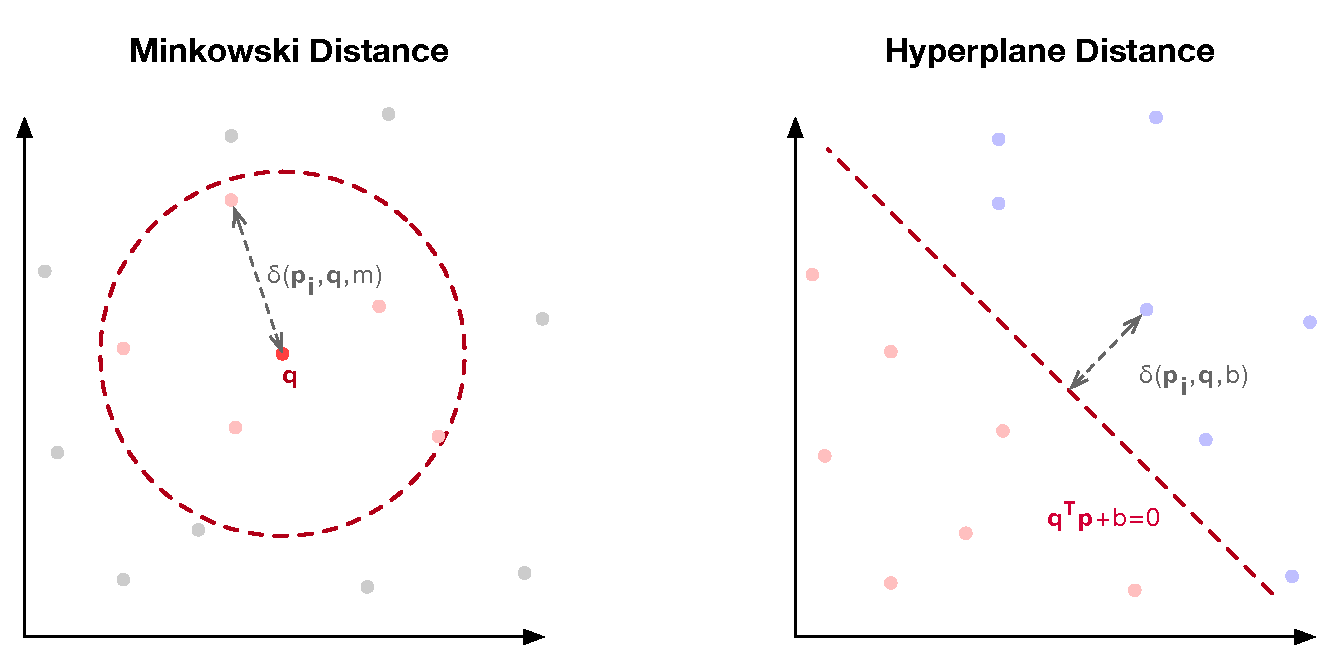
\includegraphics[width=\textwidth]{figures/distance_computations.eps}
    \caption{Two examples of distance functions that fall into the broader category of a \acrshort{dfc}. On the left, the point-distance between $q$ and $p_i$ and on the right, the distance between a hyperplane $q^Tx+b = 0$ and points $p_i$.}
    \label{figure:distance_computation}
\end{figure}

As an aside, we must address the role of dimensionality $dim$ in the case of data domains that are subsets of vector spaces, i.e.,  $\domain_q \subset \mathbb{R}^{dim}$ or $\domain_q \subset \mathbb{C}^{dim}$. One could argue, that the dimensionality of such a vector space can also be seen as a parameter of the \acrshort{dfc}. Irrespective of the merits such an argument might have, we consider the dimensionality of the vector space to be a strictly structural property of the underlying data domain $\domain_q$ and thus thightly coupled to the data type. This means, that dimensionality as well as the data type are well-defined and remain constant within and, for most parts, even between queries for a given relation.

\subsection{Extending the Relational Model}

Using \cref{definition:dfc}, one can start to integrate \acrshort{dfc} into the relational data model. Following~\cite{Giangreco:2018thesis}, we first assume  $\domainset$ -- the set system of data domains supported by the database -- to be extended by whatever data domain $\domain_q$ is required. Following that recipe, a \acrshort{dbms} can be extended to support every type of (mathematical) object that is useful for a given application, such as but not limited to $\mathbb{R}^{dim}$ or $\mathbb{C}^{dim}$. 

We now use the idea of an extended projection $\pi_{\mathcal{E}}$ -- as proposed by \cite{Gupta:1995Generalized,Garcia:2009Database} and introduced in \cref{section:relational_data_model} -- wherein $\mathcal{E}$ is simply a list of expressions involving attributes $\attribute_i \in \relation$. That is, in addition to the simple projection onto attributes $\attribute_i$, an extended projection may also include the evaluation of algebraic and function expressions. Assuming that a function invocation involving constants as well as arguments from the underlying relation are supported, the evaluation of a \acrshort{dfc} can be expressed as follows:

\begin{definition}[label=definition:spf_rel]{\acrlong{dfc} in Extended Projection $\pi_{\mathcal{E}}$}{}
    Let $\symdfc \colon \domain_q \times \domain_q \times \domain_{1} ... \times \domain_{N-2} \to \mathbb{R}$ be a N-ary \acrshort{dfc} and $\delta = \mathtt{IMP}(\symdfc)$ its implementation. Let further $\relation$ be a relation with attribute $\mathcal{A}_p \in \mathtt{SCH}(\relation)$. The \emph{extended projection} $\pi_{\delta(\mathcal{A}_p)}(\relation)$ describes the evaluation of $\delta$ using argument values $p_{i} \in \mathcal{A}_p$ as probing arguments. Applying $\pi_{\delta(\mathcal{A}_p)}$ on a M-ary relation $\relation$ introduces a new distance attribute $\mathcal{A}_d$, i.e., $\mathtt{SCH}(\pi_{\delta(\mathcal{A}_p), \mathcal{A}_1, ..., \mathcal{A}_M}(\relation)) = \mathtt{SCH}(\relation) \cup \{ \mathcal{A}_d \}$
\end{definition}

Obviously, the evaluation of multiple \acrshort{dfc}s in a single, extended projection or the combination of simple attribute projections with the evaluation of \acrshort{dfc}s are also allowed. In fact, all of the following expressions are valid examples of the extended projection on relation $\relation$ with $\mathtt{SCH}(\relation) = \{ \mathcal{A}_1, \mathcal{A}_2, \mathcal{A}_3, \mathcal{A}_4 \}$ and $\delta_i = \mathtt{IMP}(\symdfc_i)$: 
\begin{enumerate*}[label=(\roman*)]
    \item Evaluation of multiple \acrshort{dfc}s with same or different probing arguments (e.g., $\pi_{\delta_1(\mathcal{A}_1), \delta_2(\mathcal{A}_1)}(\relation)$), 
    \item evaluation of same \acrshort{dfc} using same or different probing arguments (e.g., $\pi_{\delta_1(\mathcal{A}_1), \delta_1(\mathcal{A}_2)}(\relation)$),
    \item combination of \acrshort{dfc}s with any attribute projection and/or algebraic expression evaluation (e.g., $\pi_{\delta(\mathcal{A}_1), \mathcal{A}_2, \mathcal{A}_4}(\relation)$).
\end{enumerate*}

In order to support sorting by (the obtained) distance, which is an essential part of many types of proximity based queries, we use the idea of a \emph{ranked relation} $\rankedrel$, as proposed by \cite{Chengkai:2005RankSQL} and described in \cref{section:rel_extensions}. A ranked relation \footnote{Mathematically speaking, ranked relations are not longer relations rather than sequences.} $\rankedrel$ exhibits an ordering of tuples $t_i \in \rankedrel$, which is induced by the ranking or scoring predicate $\mathcal{O}$. As opposed to \cite{Chengkai:2005RankSQL} and more in line with \cite{Garcia:2009Database}, we assume $\mathcal{O}$ to be a simple sequence of pairs $(\attribute_i, \mathtt{DIR})$ with $\mathtt{DIR} \in \left\{ \uparrow, \downarrow \right\}$ and $\attribute_i \in \rankedrel$ each denoting an attribute to order by and the desired sort direction \emph{ascending} or \emph{descending}\footnote{We argue that formally, the evaluation of a \emph{scoring function}, as proposed by \cite{Chengkai:2005RankSQL}, can be expressed within the scope of the extended projection and does not need to be part of the order operation.}. If $\relation$ does not exhibit a specific ranking, then the $\mathcal{O}$ is simply ommitted.

In order to sort an (unordered) relation, we introduce the relational operator $\tau_{\mathcal{O}}$ such that:

\begin{equation}
    \label{equation:rel_alg_tau}
    \tau_{\mathcal{O}}(\relation) = \rankedrel
\end{equation}

Again using the relation $\relation$ with $\mathtt{SCH}(\relation) = \{ \mathcal{A}_1, \mathcal{A}_2, \mathcal{A}_3, \mathcal{A}_4 \}$, the application of $\tau_{((\attribute_1,\uparrow),(\attribute_2,\downarrow))}$ on relation $\relation$ sorts the tuples $t_i \in \relation$ based on $\attribute_1$ in ascending order and breaks ties sorting by $\attribute_2$ in descending order. Tuples that are equal in both attributes appear in an arbitrary order.

So as to be able to execute a specific type of proximity based query -- namely, \acrshort{knn} or \acrshort{kfn} -- we require one last extension to the relational algebra in the form of the k-selection operator $\lambda_k(\relation)$. The $\lambda_k(\relation)$ operator simply limits the cardinality of a relation $\relation$ to $k$ tuples, without changing the order of a ranked relation $\rankedrel$. It is trivial to see that for a ranked relation $\rankedrel$, $\lambda_k(\rankedrel)$ limits the sequence of tuples to the top $k$ results w.r.t. to the ordering induced by $\mathcal{O}$.

We can now use the example presented in \cref{example:rel_painting_w_features} to demonstrate the flexibility of the proposed algebra extensions and the different types of queries that can be expressed through $\pi_{\mathcal{E}}$, $\tau_{\mathcal{O}}$, $\lambda_k$.

\begin{example}[label=example:rel_painting_w_features]{Relation listing paintings with feature vectors}{}
    
    $\relation_{p}$ lists paintings with their title $\mathcal{A}_{t}$, the year of their creation $\mathcal{A}_{y}$ and some arbitrary feature vector $\mathcal{A}_{f}$. Note that $\domain_{f} \subset \mathbb{R}^{3}$.
        
    \begin{center}
        \begin{tabular}{ l || l | l | l |}
            $\relation_{p}$ & $\mathcal{A}_{t}$  & $\mathcal{A}_{y}$  & $\mathcal{A}_{f}$ \\ 
            \hline
            \hline
            $t_1$ & Mona Lisa & 1506 & $\left\lbrack 0.0, 0.2, -1.3 \right\rbrack$ \\
            \hline
            $t_2$ & The Starry Night & 1889 & $\left\lbrack 1.0, 0.9, 2.6 \right\rbrack$ \\
            \hline
            ... & ... & ... & ... \\
            \hline
            $t_N$ & Las Meninas & 1665 & $\left\lbrack -0.5, 3.0, 0.8 \right\rbrack$ \\
            \hline
        \end{tabular}
    \end{center}

    Using \acrshort{dfc}s and the proposed, relational algebra,  we can now express:

    \begin{center}
        \begin{tabular}{||l l r ||} 
         \hline
         Name & Result & Algebraic Form \\
         \hline\hline
         \acrshort{nns} / \acrshort{kfn} & $\relation^{(\mathcal{A}_d,\uparrow)}$ & $\lambda_k (\tau_{(\mathcal{A}_d,\uparrow)} ( \pi_{\mathcal{A}_{y}, \delta(\mathcal{A}_{f})}  ( \relation_p)))$  \\ 
         \hline
         \acrshort{fns} / \acrshort{knn}& $\relation^{(\mathcal{A}_d,\downarrow)}$ & $\lambda_k (\tau_{(\mathcal{A}_d,\downarrow)} ( \pi_{\mathcal{A}_{y}, \delta(\mathcal{A}_{f})}  ( \relation_p)))$   \\
         \hline
         $\epsilon$NN & $\relation^{(\mathcal{A}_d,\uparrow)}$ & $\tau_{(\mathcal{A}_d,\uparrow)} ( \sigma_{\mathcal{A}_d \leq \epsilon} ( \pi_{\mathcal{A}_{y}, \delta(\mathcal{A}_{f})} ( \relation_p)) )$  \\
         \hline
         \acrshort{nns} w. selection & $\relation^{(\mathcal{A}_d,\uparrow)}$ &  $\tau_{(\mathcal{A}_d,\uparrow)} ( \pi_{\mathcal{A}_{year}, \delta(\mathcal{A}_{f})} ( \sigma_{\mathcal{A}_{y} = 1889} ( \relation_p)) )$\\
         \hline
         Multi order & $\relation^{(\mathcal{A}_{d1},\uparrow),(\mathcal{A}_{d2},\uparrow)}$ & $\tau_{(\mathcal{A}_{d1},\uparrow),(\mathcal{A}_{d2},\uparrow)} ( \pi_{\delta_1(\mathcal{A}_{f}), \delta_2(\mathcal{A}_{f})}  ( \relation_p))$ \\ 
         \hline
         DFS \& aggregate & $\relation$ & \\ 
         \hline
        \end{tabular}
    \end{center}

\end{example}

\subsubsection{Algebraic Properties of $\pi$, $\tau_{\mathcal{O}}$, $\lambda_k$}

During the logical optimization phase of query planning, a \acrshort{dbms} leverages the algebraic properties of the operators it employs in an attempt to generate a more efficient execution plan. Most importantly, these properties determine the types of operations that can be permuted or even exchanged. As opposed to classical relational algebra, we must consider:
\begin{enumerate*}[label=(\roman*)]
     \item Whether a permutation  
\end{enumerate*}

\todo[inline]{Elaborate on algebraic properties of $\pi$, $\tau_{\mathcal{O}}$, $\lambda_k$}

\subsubsection{Combination with Other Extensions}

\todo[inline]{Elaborate on how $\pi$, $\tau_{\mathcal{O}}$, $\lambda_k$ can be combined with other relational extensions}

\subsection{\acrshort{dfc}s and Query Planning}
\label{section:dfc_and_planning}

The requirements imposed on the structure of a \acrshort{dfc} can be leveraged to enable a \acrshort{dbms} to plan and optimize the execution of a proximity based query by not just altering the execution plan in terms of (relational) operators but also in terms of \acrshort{dfc} implementations that should be employed. To illustrate this, we proposed the notion of the \emph{function hierarchy} depicted in \ref{figure:function_hierarchy}.

\begin{figure}[bt]
    \centering
    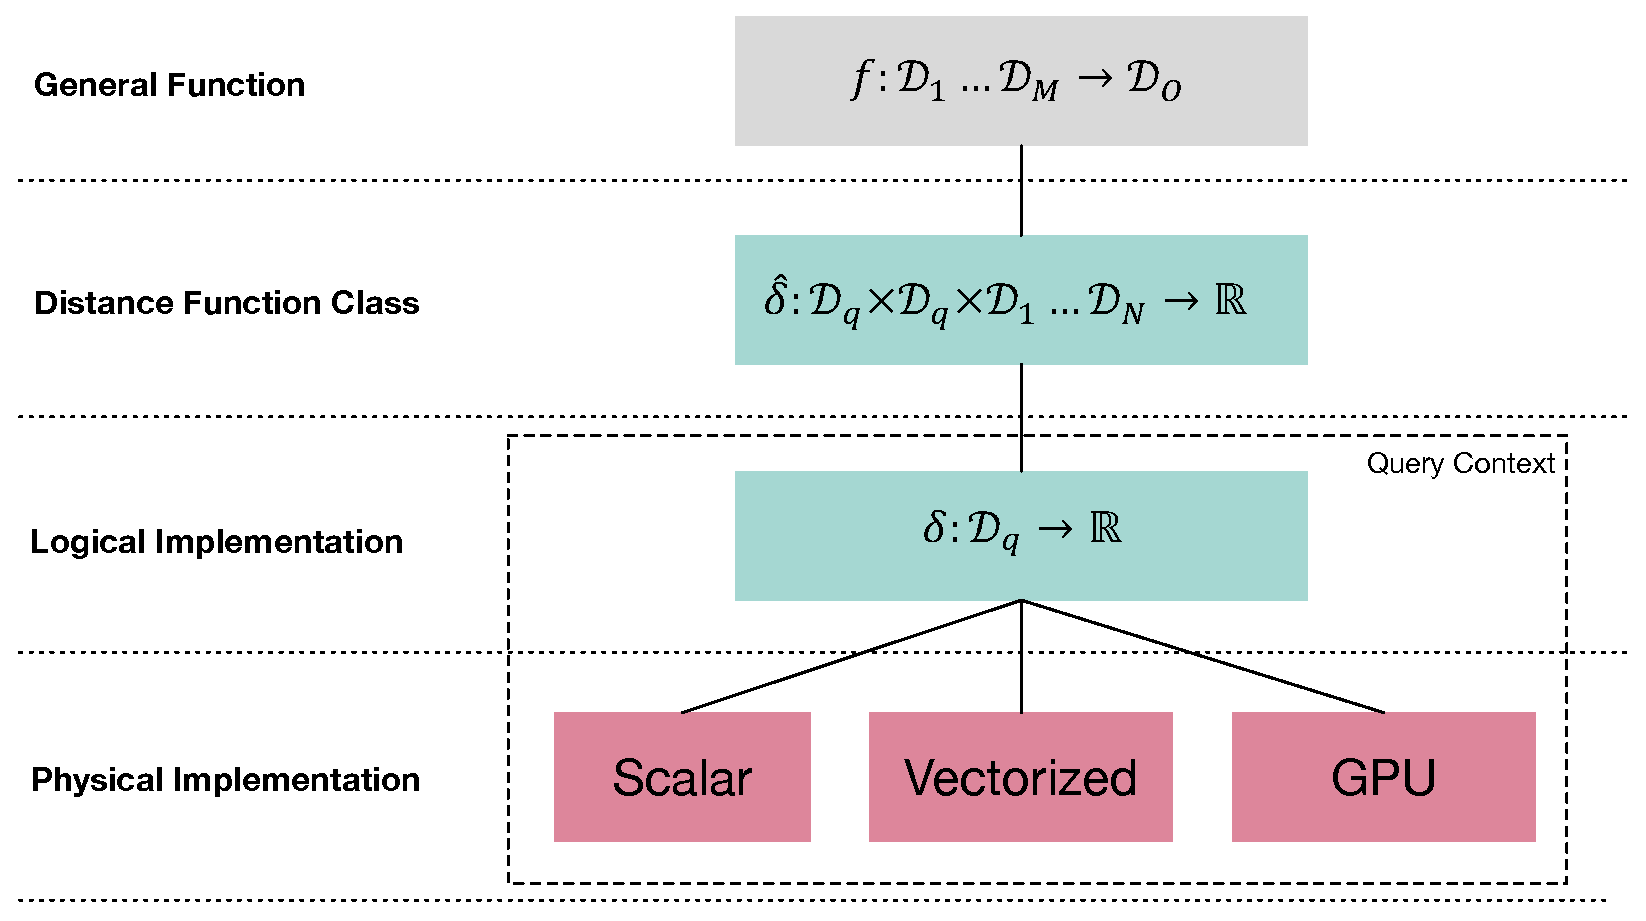
\includegraphics[width=\textwidth]{figures/function_hierarchy.eps}
    \caption{Two examples of distance functions that fall into the broader category of a \acrshort{dfc}. On the left, the point-distance between $q$ and $p_i$ and on the right, the distance between a hyperplane $q^Tx+b = 0$ and points $p_i$.}
    \label{figure:function_hierarchy}
\end{figure}

The figure depicts executable functions from a perspective of the \acrshort{dbms} and the amount of insights it has about them. At the very top, we see general functions such as \acrshort{udf}s. In general, the \acrshort{dbms} has little to no knowledge about the internals of these functions and can thus only provide very limited support for optimizing their execution. As we move down the hierarchy, the \acrshort{dbms} ``gains'' insights with respect to the function's properties. At the level of the \acrshort{dfc}, the \acrshort{dbms} is aware of the function's name and the general structure of the \acrshort{dfc}s domain and codomain. 


\todo[inline]{Elaborate on how the structure of a \acrshort{dfc} can be exploited for query planning}


\section{Cost Model for Retrieval Accuracy}
Describe cost model for execution plans with following properties:

\begin{itemize}
    \item Cost as a function of atomic costs: $f(a_{cpu}, a_{io}, a_{memory}, a_{accuracy}) \longrightarrow C$
    \item Means to estimate results accuracy and associated considerations from execution path (e.g., when using index) based on properties of the index
    \item Means to specify importance of accurate results (e.g., global, per-query, context-based i.e. when doing 1NN search) in comparison to other factors
    \item Systems perspective 1: How can such a cost model be applied during query planning and optimization?
\end{itemize}

\section{Adaptive Index Management}

\begin{figure}[h!]
    \centering
    \begin{subfigure}[b]{0.40\textwidth}
        \centering
        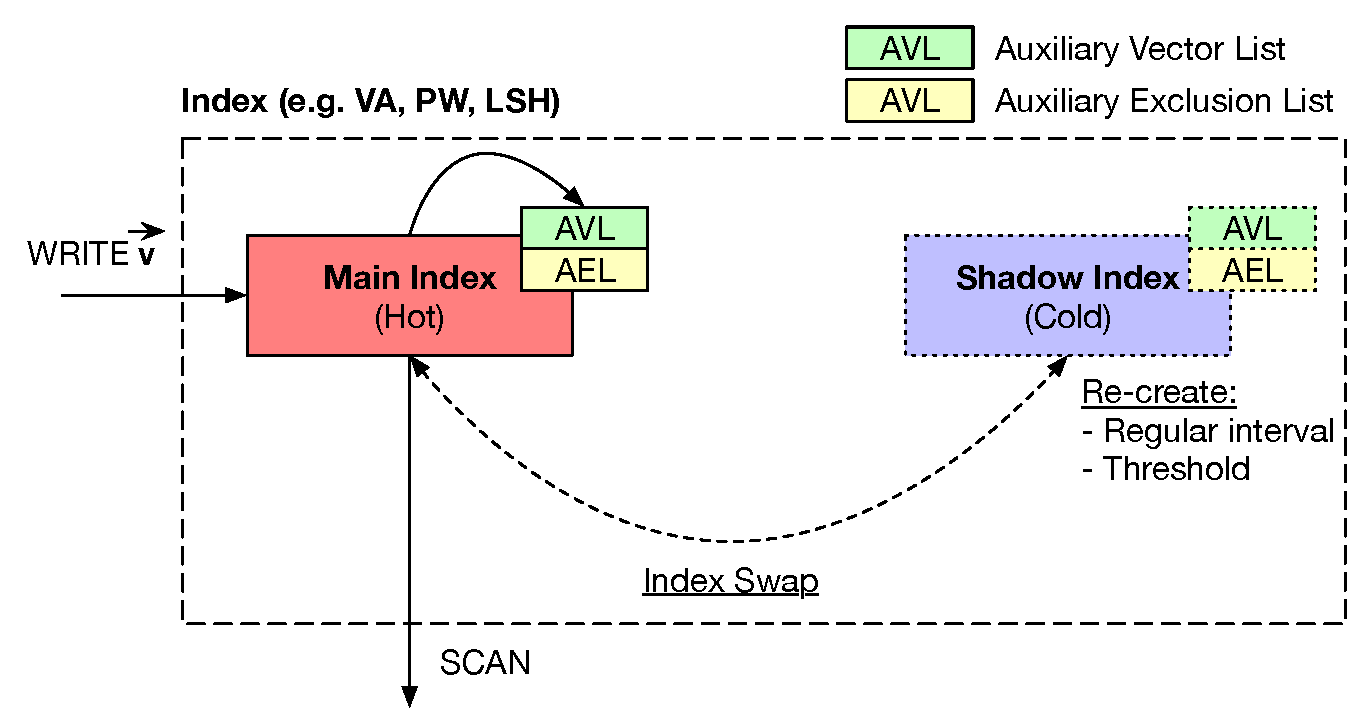
\includegraphics[width=\textwidth]{figures/adaptive_index.eps}
        \label{fig:adaptive_index:architecture}
    \end{subfigure}
    \hfill
    \begin{subfigure}[b]{0.40\textwidth}
        \centering
        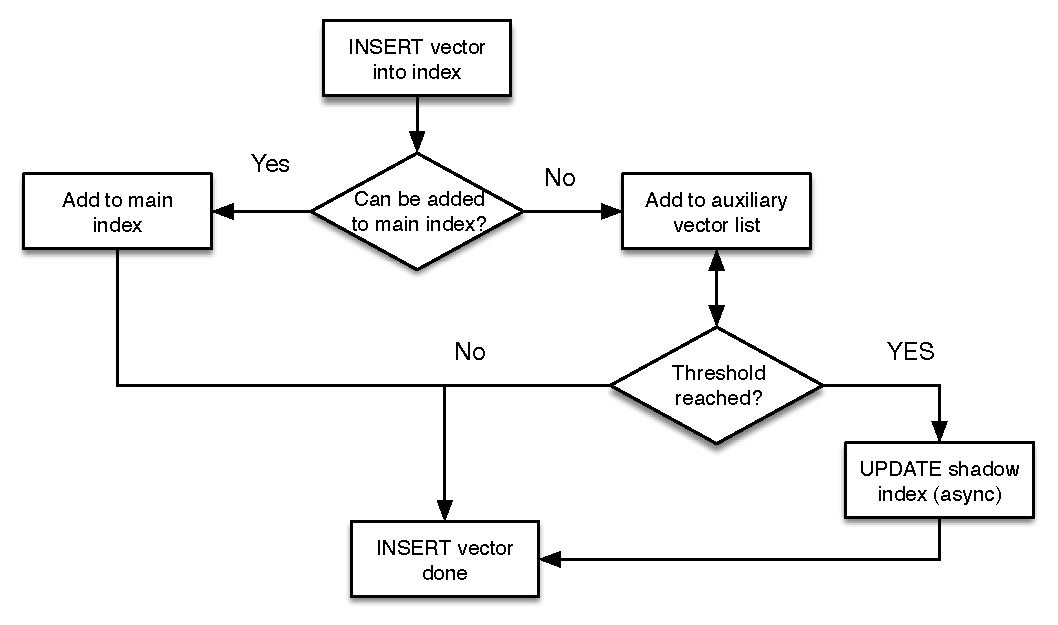
\includegraphics[width=\textwidth]{figures/adaptive_index_flow.eps}
        \label{fig:adaptive_index:flow}
    \end{subfigure}
    \caption{Adaptive index structures overview.}
    \label{fig:adaptive_index}
\end{figure}

Describe model for index management in the face of changing data (adaptive index management):

\begin{itemize}
    \item Reason about properties of secondary indexes for NNS (e.q., PQ, VA, LSH) with regards to data change
    \item Derivation of error bounds possible (e.g., usable for planning)?! Use in query planning?
    \item Systems perspective 1: How to cope with ``dirty'' indexes? Proposal: hot vs. cold index, auxilary data structure, offline optimization, see \cref{fig:adaptive_index}
    \item Systems perspective 2: On-demand index based on query workload?
\end{itemize}

\section{Architecture Model}

\todo[inline]{Putting everything together into a unified systems model (base on previous work + aforementioned aspects).}




